\begin{frame}{Proof Systems}

	$L \subseteq \{0, 1\}^*$. $\UNSAT$ is a language of unsatisfiable boolean CNF formulas.
    \pause

    \begin{definition}[Cook, Reckhow 79]
        Proof system for $L \Leftrightarrow$ poly-time algorithm
        $\Pi\colon \{0, 1\}^* \times \{0, 1\}^* \rightarrow \{0, 1\}$:
        \begin{itemize}
            \item (completeness) $x \in L \Rightarrow \exists w ~ \Pi(x, w) = 1$;
            \item (soundness) $\exists w ~ \Pi(x, w) = 1 \Rightarrow x \in L$.
        \end{itemize}
    \end{definition}

    Length of $|w|$ is the complexity measure.

    \pause

    \begin{block}{Cook's Program}
        Prove superpolynomial lower bounds for stronger and stronger proof systems until the techniques
        are developed to do it in a general case.

        Goal: $\NP \neq \coNP$.
    \end{block}
\end{frame}

\begin{frame}{Proof Systems}

    \deftext{Resolution}: proof of $\varphi \coloneqq \bigwedge\limits_{i} C_i$ is a sequence of clauses
    $(D_1, D_2, D_3, \dots, D_{\ell})$:
    \pause
    
    \begin{minipage}{0.3\linewidth}
        \begin{itemize}
            \item $D_i \in \{C_i\}$;
                \pause
            \item $\frac{A \lor x ~~~~~ B \lor \bar{x}}{A \lor B}$, $D_i \coloneqq A \lor B$;
                \pause
            \item $D_{\ell} = \emptyset$.
        \end{itemize}
    \end{minipage}
    \pause
    \begin{minipage}{0.68\linewidth}
        \centering
        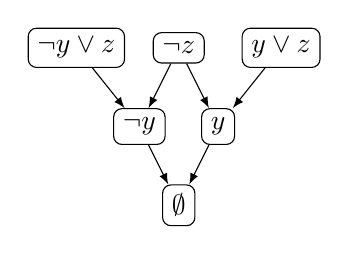
\begin{tikzpicture}[>=latex]
    \node[rectangle, rounded corners = 3pt, draw] (a) at (-1.3, 2)
        {$\neg y \lor z$};
    \node[rectangle, rounded corners = 3pt, draw] (a2) at (1.3, 2)
        {$y \lor z$};
    \node[rectangle, rounded corners = 3pt, draw] (b) at (0, 2)
        {$\neg z$};
    \node[rectangle, rounded corners = 3pt, draw] (c) at (-0.5, 1)
        {$\neg y$};
    \node[rectangle, rounded corners = 3pt, draw] (d) at (0.5, 1)
       {$y$};
    \node[rectangle, rounded corners = 3pt, draw] (e) at (0, 0)
        {$\emptyset$};

    \draw[->] (a) -- (c);
    \draw[->] (a2) -- (d);
    \draw[->] (b) -- (c);
    \draw[->] (b) -- (d);
    \draw[->] (c) -- (e);
    \draw[->] (d) -- (e);
\end{tikzpicture}
    \end{minipage}


    \pause
    \vspace{0.3cm}

    \deftext{Cutting Planes}: proof is a sequence of inequalities over $\mathbb{Z}$
    $(p_1 \ge 0, p_2 \ge 0, p_3 \ge 0, \dots, p_{\ell} \ge 0)$:
    \begin{itemize}
        \item $p_i$ is an encoding of $C \in \varphi$, $x_k \ge 0$ or $-x_k + 1 \ge 0$;
        \item $\frac{p_i ~~~~~ p_j}{p_k}$,  $(p_i \ge 0) \land (p_j \ge 0)$ imply $(p_k \ge 0)$
            \alert{over $\mathbb{Z}^n$};
        \item $p_{\ell} = 1$.
    \end{itemize}

    \pause
    \vspace{0.3cm}

    \deftext{Nullstellensatz}: proof of a system of polynomial equalities $f_1 = 0, f_2 = 0, \dots$:
    $$
        \sum_{u = 1}^{a} p_u f_u = 1.
    $$
\end{frame}


\begin{frame}{Pebbing}

    \begin{center}
        \tikzstyle{vert} = [
    circle,
    draw,
    inner sep = 0pt,
    minimum size = 0.45cm,
    fill = LEIorange!5
]
\tikzstyle{pstyle} = [alt=<{#1}>{fill = LEIorange!50}{}]
    
\tikzset{
    xcenter around/.style 2 args = {
        execute at end picture = {%
            \useasboundingbox let \p0 = (current bounding box.south west),
            \p1 = (current bounding box.north east),
            \p2 = (#1),
            \p3 = (#2) in ({min(\x2 + \x3 - \x1, \x0)}, \y0) rectangle ({max(\x3 + \x2 - \x0, \x1)},\y1);
        }
    }
}

\begin{tikzpicture}[>=latex, xcenter around = {-2.1, -2.1}{2.1, 0.1}]
    \node at (3.6, -0.6) {\includegraphics[scale = 0.09]{pics/utia-rest.png}};
    
    \node[vert, pstyle = 2] (a) at (0, 0) {$r$};
    \node[vert, pstyle = 4] (b) at (-1, -1) {$x$};
    \node[vert] (c) at (1, -1) {$y$};
    \node[vert, pstyle = {3-4}] (d) at (-2, -2) {$z$};
    \node[vert, pstyle = {3-4}] (e) at (0, -2) {$u$};
    \node[vert, pstyle = 3] (f) at (2, -2) {$w$};

    \draw[->] (b) -- (a);
    \draw[->] (c) -- (a);
    \draw[->] (d) -- (b);
    \draw[->] (e) -- (b);
    \draw[->] (e) -- (c);
    \draw[->] (f) -- (c);
\end{tikzpicture}        
    \end{center}

    \pause
    \begin{itemize}
        \item $(\neg r)$;
            \pause
        \item $(z), (u), (w)$;
            \pause
        \item $(\neg z \lor \neg u \lor x)$.    
    \end{itemize}

    \pause
    \tikzset{
    pr-vert/.style = {
        draw,
        rounded rectangle,
        minimum width = 1cm,
        minimum height = 0.4cm,
        outer sep = 0pt,
        fill = #1
    },
    pr-vert/.default = LEIblue!10
}

\tikzstyle{ops} = [alt = <{#1-}>{opacity = 1}{opacity = 0}]

\begin{tikzpicture}
    \node[pr-vert, ops = 6] (a) at (0, 0) {$u$};
    \node[pr-vert, ops = 6] (b) at (0, -1) {$z$};
    \node[pr-vert, ops = 6] (c) at (0, -2) {$\neg z \lor \neg u \lor x$};
    
    \node[pr-vert = LEIorange!10, ops = 7] (d) at (2, -1.9) {$\neg u \lor x$};
    \node[pr-vert = LEIorange!10, ops = 7] (e) at (3, -1.25) {$x$};

    \node[pr-vert, ops = 8] (f) at (4, 0) {$\neg u \lor \neg w \lor y$};
    \node[pr-vert, ops = 8] (g) at (6, 0) {$w$};
    
    \node[pr-vert = LEIorange!10, ops = 8] (h) at (5, -0.75) {$\neg w \lor y$};
    \node[pr-vert = LEIorange!10, ops = 8] (i) at (6.5, -1) {$y$};

    \node[pr-vert, ops = 9] (j) at (5, -2) {$\neg x \lor \neg y \lor r$};

    \node[pr-vert = LEIorange!10, ops = 9] (k) at (7.5, -2) {$\neg y \lor r$};
    \node[pr-vert = LEIorange!10, ops = 9] (l) at (8.5, -1.2) {$r$};

    \node[pr-vert, ops = 10] (m) at (8.5, 0) {$\neg r$};

    \node[pr-vert = red!30, ops = 10] (n) at (9.5, -0.6) {$\emptyset$};

    \draw[->, ops = 7] (b) -- (d);
    \draw[->, ops = 7] (c) -- (d);
    \draw[->, ops = 7] (a) -- (e);
    \draw[->, ops = 7] (d) -- (e);

    \draw[->, ops = 8] (a) -- (h);
    \draw[->, ops = 8] (f) -- (h);
    \draw[->, ops = 8] (h) -- (i);
    \draw[->, ops = 8] (g) -- (i);

    \draw[->, ops = 9] (e) -- (k);
    \draw[->, ops = 9] (j) -- (k);
    \draw[->, ops = 9] (k) -- (l);
    \draw[->, ops = 9] (i) -- (l);

    \draw[->, ops = 10] (l) -- (n);
    \draw[->, ops = 10] (m) -- (n);
\end{tikzpicture}
\end{frame}

\begin{frame}{Motivation}

    \begin{itemize}
        \item If there is no short proofs of unsatisfiability $\Rightarrow$ no poly-time algorithm for
            $\SAT$ and $\P \neq \NP$.
        \pause
        \item Resolution lower bounds $\Rightarrow$ explicit hard examples for some classes of algorithms
            for $\SAT$.
        \pause
        \item Weak proof systems (Resolution etc.) lower bounds $\Rightarrow$ explicit hard examples for
            \alert{monotone} computations.
    \end{itemize}

    \pause
    \vspace{1cm}
    \begin{block}{Remark}
        For some applications we should prove lower bounds on the specific formulas.        
    \end{block}
\end{frame}


\begin{frame}{$\DPLL$ Algorithms}

    \begin{center}
        \onslide<1->{
   	\tikzstyle{vertex2} = [opacity = 0]
   	\tikzstyle{vertex3} = [opacity = 0]
    \tikzstyle{vertex4} = [opacity = 0]
   	\tikzstyle{vertex5} = [opacity = 0]
    \tikzstyle{vertex9} = [opacity = 0]
    \tikzstyle{vertex11} = [opacity = 0]
}
\only<2->{\tikzstyle{vertex2} = [opacity = 1]}
\only<3->{\tikzstyle{vertex3} = [opacity = 1]}
\only<4->{\tikzstyle{vertex4} = [opacity = 1]}
\only<5->{
  	\tikzstyle{vertex5} = [opacity = 1]
    \tikzstyle{vertex9} = [opacity = 1]
}

\tikzstyle{end} = [circle, minimum size = 0.6cm, draw = black, inner sep = 0.1pt]
            
\tikzstyle{level 1} = [draw = black, level distance = 1.5cm, sibling distance = 5cm]
\tikzstyle{level 2} = [sibling distance = 2cm]
    
\begin{tikzpicture}[label distance=8mm]
	\node [end] (z){$\varphi$}
		child [vertex2] {
    		node [end] (b) {$\varphi'$}
			child [vertex3]{
	           	node {$\vdots$}
                edge from parent
	  	        node[left] {$w \coloneqq 0$}
            }
		    child [vertex4]{
            	node[end] {$\varphi''$}
            	child [vertex4]{
            	   	node {$\vdots$}
            		edge from parent
	  	        	node[left] {$y \coloneqq 0$}
                }
                child [vertex4]{
            	   	node {$\vdots$}
            		edge from parent
	  	        	node[right] {$y \coloneqq 1$}
            	}
                edge from parent
	   	        node[right] {$w \coloneqq 1$}
            }
           	edge from parent
            node[above left] {$x \coloneqq 0$}
        }
        child [vertex5] {
        	node [end] (c) {$\varphi'''$}
           	child [vertex9]{
               	node {$\vdots$}
                edge from parent
	            node[left] {$z \coloneqq 0$}
            }
		    child [vertex9]{
               	node {$\vdots$}
                edge from parent
	            node[right] {$z \coloneqq 1$}
            }
            edge from parent
	   	    node[above right] {$x \coloneqq 1$}
        };
\end{tikzpicture}        
    \end{center}

    
	\pause
    \pause
    \pause
    \pause
    \pause
    \begin{itemize}
        \item Heuristic $\mathbf{A}$ chooses a variable for splitting.
    	\pause
	    \item Heuristic $\mathbf{B}$ chooses the first value.
    	\pause
    	\item Simplification rules: \alert{no simplifications!}
    \end{itemize}
\end{frame}

\begin{frame}{$\DPLL$ and Resolution}
    
    \begin{theorem}
        $\DPLL$ algoritm makes $t$ splitting on \alert{unsatisfiable} CNF formula
        $$\varphi \coloneqq \bigwedge\limits_i C_i$$
        $\Rightarrow$ there exists a resolution proof of $\varphi$ of size $2t$.
    \end{theorem}

    \pause

    \begin{minipage}{0.58\linewidth}
        \centering
        \tikzstyle{inner} = [circle, minimum size = 0.3cm, draw, inner sep = 0.1pt]
\tikzstyle{gstyle} = [fill = green]
\tikzstyle{rstyle} = [fill = red]
\tikzstyle{ed} = [->, draw]
\tikzstyle{ops} = [alt=<{#1-}>{opacity = 1}{opacity = 0}]
\tikzstyle{opstyle} = [inner, ops = #1]
\tikzstyle{oped} = [ed, ops = #1]
\tikzstyle{gstyle} = [alt=<{#1}>{fill = green}{}]
\tikzstyle{rstyle} = [alt=<{#1}>{red!90!black}{}]
\tikzstyle{snakestyle} = [
    alt=<{#1}>{
        decorate,
        decoration = {
            snake,
            amplitude = 0.4mm,
            segment length = 2mm,
            post length = 1mm
        }
    }{}]


    
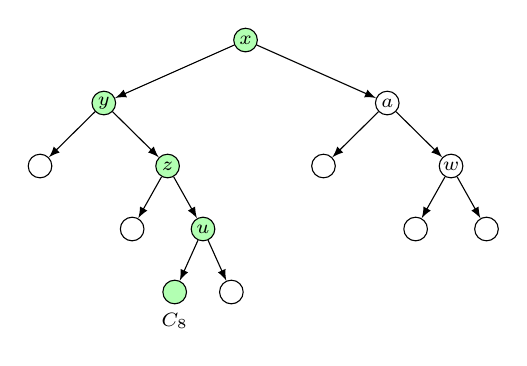
\begin{tikzpicture}[>=latex, xscale = 0.9]
    
    \node[inner, fill = green!30] (a) at (0, 0) {\scriptsize $x$};
    \node[inner, fill = green!30] (b) at (-2, -0.8) {\scriptsize $y$};
    \node[inner] (c) at (2, -0.8) {\scriptsize $a$};
    \node[inner] (d) at (-2.9, -1.6) {};
    \node[inner, fill = green!30] (e) at (-1.1, -1.6) {\scriptsize $z$};
    \node[inner] (f) at (1.1, -1.6) {};
    \node[inner] (g) at (2.9, -1.6) {\scriptsize $w$};

    \node[inner] (h) at (-1.6, -2.4) {};
	\node[inner, fill = green!30] (i) at (-0.6, -2.4) {\scriptsize $u$};
    
    \node[inner] (j) at (2.4, -2.4) {};
    \node[inner] (k) at (3.4, -2.4) {};

    \node[inner, fill = green!30] (l) at (-1, -3.2) {};
    \node[below = 4pt] at (l) {\scriptsize $C_{8}$};
    \node[inner] (m) at (-0.2, -3.2) {};
    
    \draw[ed] (a) -- (b);
    \draw[ed] (a) -- (c);
    \draw[ed] (b) -- (d);
    \draw[ed] (b) -- (e);
    \draw[ed] (c) -- (f);
    \draw[ed] (c) -- (g);
    \draw[ed] (e) -- (h);
    \draw[ed] (e) -- (i);
    \draw[ed] (g) -- (j);
    \draw[ed] (g) -- (k);
    \draw[ed] (i) -- (l);
    \draw[ed] (i) -- (m);
\end{tikzpicture}
    \end{minipage}
    \pause
    \begin{minipage}{0.4\linewidth}
        \centering
        $\frac{A \lor x ~~~ B \lor \neg x}{A \lor B} ~~~~~ \frac{A}{A \lor z}$
        \begin{itemize}
            \item Node $\Rightarrow$ disjunction of negations of queries.
            \item $(x \lor \neg y \lor \neg z \lor u)$.
        \end{itemize}
    \end{minipage}

\end{frame}

\begin{frame}{Lower bounds in proof complexity}

    
\tikzset{
    vert/.style = {
        draw,
        ellipse
    },
    tikzart-fire/.pic = {
        \draw[fill = red!60] (0, 0) .. controls (0.3, 0) and (0.6, 0.1) .. (0.7, 0.3)
            .. controls (0.8, 0.5) and (0.85, 0.6) .. (0.8, 0.9)
            .. controls (0.75, 1.1) and (0.7, 1.2) .. (0.6, 1.4)
            .. controls (0.65, 1.2) and (0.6, 1.05) .. (0.5, 0.9)
            .. controls (0.5, 1.2) and (0.2, 1.3) .. (0.1, 1.6)
            .. controls (0.05, 1.75) and (0.1, 2) .. (0.2, 2.1)
            .. controls (-0.1, 2) and (-0.2, 1.85) .. (-0.3, 1.7)
            .. controls (-0.4, 1.5) and (-0.45, 1.3) .. (-0.4, 1.1)
            .. controls (-0.5, 1.2) and (-0.51, 1.4) .. (-0.5, 1.5)
            .. controls (-0.75, 1.2) and (-0.8, 0.7) .. (-0.7, 0.5)
            .. controls (-0.6, 0.28) and (-0.4, 0) .. (0, 0);
            \fill[white] (0, 0) .. controls (0.3, 0) and (0.52, 0.34) .. (0.37, 0.61)
            .. controls (0.4, 0.54) and (0.32, 0.32) .. (0.25, 0.25)
            .. controls (0.3, 0.35) and (0.25, 0.5) .. (0.2, 0.6)
            .. controls (0.1, 0.8) and (-0.05, 1) .. (0, 1.2)
            .. controls (-0.32, 1) and (-0.3, 0.72) .. (-0.2, 0.47)
            .. controls (-0.3, 0.51) and (-0.31, 0.6) .. (-0.33, 0.7)
            .. controls (-0.4, 0.6) and (-0.4, 0.5) .. (-0.4, 0.4)
            .. controls (-0.35, 0.18) and (-0.2, 0) .. (0, 0);
    },
    semisim/.style = {
        ->,
        blue,
        dashed,
        decorate,
        decoration = {
            snake,
            amplitude = 0.5,
            segment length = 2
        }
    },        
}


    
\begin{tikzpicture}[xscale = 1.3, xshift = -1]
    \node[vert] (res) at (1, 0) {$\Res$};
    \node[vert] (ns) at (-3, 0) {$\NS$};
    \node[vert] (cp) at (3, 1) {$\CP$};
    \node[vert] (resk) at (1.2, 1.4) {$\Res(k)$};
    \node[vert] (acf) at (1.3, 2.4) {$\AC_0$-Frege};
    \node[vert] (resl) at (-1.3, 2.7) {$\ResL$};
    \node[vert] (acfp) at (0.5, 3.8) {$\AC_0[p]$-Frege};
    \node[vert] (fre) at (0.5, 5) {Frege};
    \node[vert] (ips) at (-2, 6) {$\PrSys{IPS}$};
    \node[vert] (pcr) at (-2.8, 1.9) {$\PCR[]$};
    \node[vert] (sos) at (-4, 2.5) {$\SOS$};
    
    \node[vert] (cps) at (-4, 6.5) {$\PrSys{CPS}$};

    

    \draw[->, semisim] (pcr) -- (sos);
    \draw[->] (res) -- (cp);
    \draw[->] (cp) to[out = 90, in = -20] (fre);
    \draw[->] (res) -- (resl);
    \draw[->] (res) -- (resk);
    \draw[->] (resk) -- (acf);
    \draw[->] (res) to[out = 138, in = -30] (pcr);
    \draw[->] (ns) -- (pcr);
    \draw[->] (resl) -- (acfp);
    \draw[->] (acf) -- (acfp);
    \draw[->] (acfp) -- (fre);
    \draw[->] (fre) -- (ips);
    \draw[->, semisim] (ips) -- (cps);

    \draw[->] (pcr) -- (ips);
    \draw[->] (sos) -- (cps);

    \node at (0, 6.9) {};
    

    \begin{scope}[on background layer]
        \draw[ultra thick, fill = black!5] (-4, -1) to[out = 110, in = 220] (-4.4, 3)
            to[out = 40, in = 180] (-1, 2) to[out = 0, in = 125] (2.3, 3) to[out = -55, in = 90]
            (1.5, -1);
    \end{scope}
    \node[blue] at (-1.5, 0.95) {Restriction};


    \begin{scope}[on background layer]
        \fill[orange!5] (-4, -1) to[out = 90, in = 180] (-2.3, 0.75) to[out = 0, in = 180] (0.5, 0.7)
            to[out = 0, in = 200] (3.5, 2) -- (3.5, -1) -- cycle;
        \draw[ultra thick, orange] (-4, -1) to[out = 90, in = 180] (-2.3, 0.75) to[out = 0, in = 180]
            (0.5, 0.7) to[out = 0, in = 200] (3.5, 2);
        \draw[ultra thick] (-4, -1) to[out = 110, in = 220] (-4.4, 3) to[out = 40, in = 180] (-1, 2)
            to[out = 0, in = 125] (2.3, 3) to[out = -55, in = 90] (1.5, -1);
    \end{scope}
    \node[blue] at (0, -0.7) {Mon. Interpolation};
\end{tikzpicture}
    
\end{frame}

\begin{frame}{Pigeonhole Principle}

    \begin{minipage}{0.4\linewidth}
        \centering
        \begin{tikzpicture}[>=latex]

    \foreach \i in {1, 2, ..., 6}{
        \node[draw, circle, fill = LEIblue!40, inner sep = 0pt, minimum size = 5pt]
            (a\i) at (0, -0.7 * \i) {};
    }

    \foreach \i in {1, 2, ..., 5}{
        \node[draw, circle, fill = LEIblue!40, inner sep = 0pt, minimum size = 5pt]
            (b\i) at (1.5, -0.7 * \i) {};
    }

    \node[below = 8pt] at (a6) {$m$};
    \node[below = 8pt] at (b5) {$n$};

    
    \draw (a4) -- (b3) node[midway, above] {$x_{i, j}$};
    \draw (a4) -- (b5) node[midway, below] {$x_{i, j'}$};
\end{tikzpicture}
    \end{minipage}
    \pause
    \begin{minipage}{0.58\linewidth}
        \begin{center}
            \includegraphics[width = .3\textwidth]{pics/pigeon3.png}
        \end{center}
        \begin{itemize}
            \item $\prod\limits_{j} x_{i, j} = 0$;
            \item $(1 - x_{i, j})(1 - x_{i', j}) = 0$.
        \end{itemize}
    \end{minipage}

    \pause
    \vspace{0.5cm}

    Another distribution, another measure, but the same idea [Razborov' 98; Alekhnovich, Razborov 03].

    \vspace{0.2cm}
    \pause
    \begin{minipage}{0.3\linewidth}
        \centering
        \begin{itemize}
            \item $m = n + 1$ \pause $\color{green!80!black}\checkmark$
        \end{itemize}
    \end{minipage}
    \pause
    \begin{minipage}{0.3\linewidth}
        \centering
        \begin{itemize}
            \item $m \ll n^2$ \pause $\color{green!80!black}\checkmark$
        \end{itemize}
    \end{minipage}
    \pause
    \begin{minipage}{0.3\linewidth}
        \centering
        \begin{itemize}
            \item $m \gg n^2$ \pause \begin{tikzpicture}
    \node[inner xsep = 0pt, inner ysep = -30pt] at (0, 0) {
        \includegraphics[width = 0.25\textwidth]{pics/pigeon4.png}
    };
    \node at (0pt, -8pt) {};
\end{tikzpicture}

        \end{itemize}
    \end{minipage}
\end{frame}
